\section{Vorlesung 21.12.2016}
\subsection{neighbor joining}
geg: Distanzmatrix (d) auf Menge X von Taxa $\rightarrow$ Baum (ungewurzelt)\\
Iteration:
\begin{enumerate}
	\item suche $argmin_{x,y} \tilde d_{xy}=\{u,v\}$
	\item ersetze $\{u,v\} \rightarrow$ no (neuer Knoten)
	\item brechne $d_{wz}$ für $z \neq u,v \rightarrow$ Schritt 1
\end{enumerate}
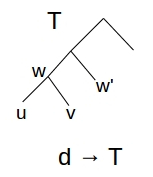
\includegraphics[width=0.2\textwidth]{lectures/161221/pix/1.jpg}\\
$\tilde d$ Transformation von d\\
F:$d \mapsto \tilde d$\\
$d_{wz}=\phi(d_{uz}, d_{vz}, d_{uz})$
\\\\
Ein Baumrekonstruktionsalgorithmus $\mathcal{A}:d \mapsto T$ ist konsistent wenn:\\
Falls d ein additive Baum-Metrik mit Baum $\hat T$ ist, dann ist $\mathcal{A}(d)=\hat T$

Beispiel:\\
$\tilde d = d$\\
$d_{wz}=\frac{1}{2} \cdot d_{uz} + \frac{1}{2} \cdot d_{vz}$ (WPGMA)\\
$d_{wz}=\frac{|u|}{|u| + |v|} \cdot d_{uz} + \frac{|u|}{|u| + |v|} \cdot d_{vz}$ (UPGMA)\\
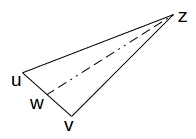
\includegraphics[width=0.4\textwidth]{lectures/161221/pix/2.jpg}\\
Ist der zugehörige Alogrithmus konsistent?\\
Gegenbeispiel:\\
$l_a,l_b,q << l_c,l_d \Rightarrow argmin_{x,y} \tilde d_{xy}=\{a,b\}$\\
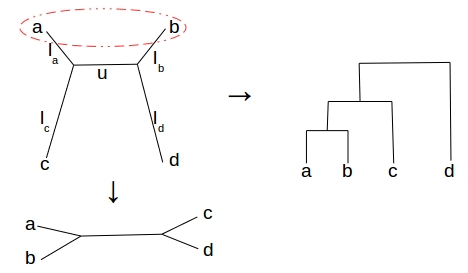
\includegraphics[width=0.7\textwidth]{lectures/161221/pix/3.jpg}\\
(Problem: LBA - long branch attraction)\\\\
Lösung:\\
Abstand eines Punktes von allen anderen Punkten berechnen:$r(u)=\displaystyle \sum_{x \neq u}d(x,u)$\\
$\tilde d_{xy}=d_{xy}-\alpha \cdot r(x) - \beta \cdot r(y)$\\
$\alpha = \beta = \frac{1}{n-2}$ mit n=Zahl der Taxa\\

\fcolorbox{red}{white}{\parbox{\linewidth}{
\textbf{Lemma:} Wenn d eine additive Baum-Metrik ist und $\{u,v\}=argmin_{x,y} \tilde d_{xy}=\{u,v\} \Rightarrow$ u,v wird cherry genannt.}}
\\\\
$\{u,v\} \mapsto w$ (u und v mittels Vaterknoten w vereinigen)\\
$d(u,w)=\frac{1}{2} \cdot d(u,v) + \frac{1}{2} \cdot \frac{1}{n-2}[r(u)-r(v)]$\\
durch Symmetrie:
$d(v,w)=\frac{1}{2} \cdot d(u,v) + \frac{1}{2} \cdot \frac{1}{n-2}[r(v)-r(u)]$\\
$d(w,z)=\frac{1}{2} \cdot [d(u,z) - d(u,w)] + \frac{1}{2} \cdot [d(v,z)-d(u,w)]$\\
$=\frac{1}{2} \cdot [d(u,z) + d(v,z)] - d(u,w)$\\

[Paper: Gascuel + Steel, Mol Biol Evol, 23 Seite 1997-2000 (2006)\footnote{\url{http://mbe.oxfordjournals.org/content/23/11/1997.long}}]
\\
\subsection{Neighbor Net}
Kalmanson Metrik\\
$\rightarrow$ zirkuläre Ordnung der Taxa\\
\begin{itemize}
	\item Auswahl der Nachbarn
	\item Update der Distanzen
\end{itemize}

\underline{Initialisierung:} Jeder Punkt ist in einem separaten Cluster C$_i$, mit Punkten x,y,…\\
$d(C_i,C_j):=\frac{1}{|C_i||C_j|} \displaystyle \sum_{\substack{x \in C_i \\ y \in C_j}}d(x,y)$\\
\\
$Q(C_i,C_j):=(m-2) \cdot d(C_i,C_j) - \displaystyle \underbrace{\sum_{k \neq i} d(C_i,C_k)}_{(m-2) \cdot r(C_i)} - \displaystyle \underbrace{\sum_{k \neq j} d(C_j,C_k)}_{(m-2) \cdot r(C_j)}$\\
mit m= Anzahl Cluster\\
(NI-Formale für Cluster)\\
Bestimme i*,j* = $argmin_{i,j} Q(C_i,C_j)$\\
$C_i,C_j$ enthält jeweils entweder 1 oder 2 Knoten\\
für Punkte in $x_i \in C_i$* und $x_j \in C_j$*\\
$\hat Q(x_i,x_j)=(\hat m -2) \cdot d(x_i,x_j) - \displaystyle \sum_{k} d(x_i,C_k) - \displaystyle \sum_{k} d(x_j,C_k)$\\
$\hat m = m - \underbrace{2}_{i*,j*} + |C_{i*}| + |C_{j*}|$\\
Erkläre x*,y* mit $x* \in C_{i*}, y* \in C_{j*}$ (mit jedem Schritt eine Kante mehr)
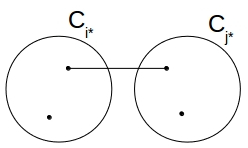
\includegraphics[width=0.5\textwidth]{lectures/161221/pix/4.jpg}\\
y hat 2 (verschiedene) Nachbarn x,z\\
a$\neq$x,y,z,u,v\\
$d(u,a)=\alpha \cdot d(x,a) + \beta \cdot d(y,a)$\\
$d(v,a)=\beta \cdot d(y,a) + \gamma \cdot d(z,a)$\\
$d(u,v)=\alpha \cdot d(x,y) + \beta \cdot d(x,z) + \gamma \cdot d(y,z)$\\
mit $\alpha + \beta + \gamma = 1;\ \alpha,\beta,\gamma \geq 0;\ \alpha=\beta=\gamma=\frac{1}{3}$\\\\
\fcolorbox{red}{white}{\parbox{\linewidth}{
\textbf{Theorem:} Wenn d Kalmanson Eigenschaften hat\\
$\Rightarrow$ Neighbor Net erzeugt die zugehörige zirkuläre Ordnung und identifiziert damit alle Splits mit nichtnegativen $\beta_{A|B}$
}}\\\\
letzter Schritt im Neighbor Net Algorithmus:\\
$\displaystyle \min_{\substack{\beta_{A|B} \forall A|B \\ cirkul\ddot{a}re\ Splits}} (\sum_{x,y} (d(x,y) - \sum_{splits} \beta_{A|B} \cdot \delta_{A|B}(x,y))^2)$ mit $\beta_{A|B} \geq 0$\\
